\documentclass[a4paper,14pt]{extarticle}
\def\source{/home/osabio/tex/templates}
\input{\source/head.tex}
\yakovlev{28}{Электростатика}
% Стыдить лжеца, шутить над дураком
% И спорить с женщиной — всё то же,
% Что черпать воду решетом:
% От сих троих избавь нас, боже!..

% М. Ю. Лермонтов.
\begin{document}

\begin{figure}[h!]
	\centering
	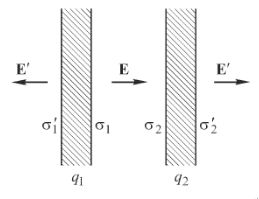
\includegraphics[width=0.4\textwidth]{img.png}
	% \caption{Caption here}
	% \label{fig:figure1}
\end{figure}

Две пластины создают поля $E_1=2\pi q_1$ и $E_2=2\pi q_2$, каждая отдельно. Тогда по принципу суперпозиции между пластинами
\begin{equation}
	\vec{E}=\vec{E}_{\sum}=\vec{E}_1+\vec{E}_2
\end{equation}
\begin{equation}
	E=2\pi(q_1-q_2)
\end{equation}
А вне пластин поля складываются:
\begin{equation}
	E'=2\pi(q_1+q_2)
\end{equation}
Возьмем цилиндр, основания которого лежат в пластинах ($E=0$ внутри проводника). Тогда для него из теоремы Гаусса следует:
\begin{equation}
	ES=0=4\pi Q=4\pi(\sigma_1+\sigma_2)S
\end{equation}
Откуда, очевидно,
\begin{equation}
	\sigma_1=-\sigma_2
\end{equation}
Теперь возьмем цилиндр, одно основание которого лежит в левой плоскости, а второе между плоскостями. Опять воспользуемся теоремой Гаусса:
\begin{equation}
	ES=2\pi(q_1-q_2)S=4\pi\sigma_1S
\end{equation}
Откуда
\begin{equation}
	\sigma_1=\frac12(q_1-q_2), \quad \sigma_2=-\frac12(q_1-q_2)
\end{equation}
Отсюда очевидно следует
\begin{equation}
	\sigma_1'=q_1-\sigma_1=q_1-\frac12(q_1-q_2)=\frac12(q_1+q_2)
\end{equation}
И аналогично
\begin{equation}
	\sigma_2'=q_2-\sigma_2=q_2+\frac12(q_1-q_2)=\frac12(q_1+q_2)
\end{equation}

% 90. а\ = -<т2 = - (q\ - q2), <т[ = <т2 = - I «0; е =

%
\end{document}